\chapter{Testing}\label{cha:testing}

% Covers unit tests, and performance tests

As discussed in Chapter \ref{cha:intro}, the main objective is to improve the speed of data processing for large datasets, making it essential to conduct performance testing of the overall system. This section aims to cover a number of methods in which the performance of the completed solution is evaluated.

%Firstly, raw performance testing is conducted against a typical data processing solution, Microsoft SQL Server. Then, a number of alternative approaches are assessed for determining how well the cluster leverages the parallelisation of running the computation over multiple nodes.



\section{Unit Tests}
Thorough unit testing is important for any software engineering focused project. By writing tests throughout development, the expected behaviour of individual components in the system can be validated. Through the use of continuous integration/continuous deployment (CI/CD) pipelines, this behaviour can continue to be validated as other parts of the system are improved, to ensure changes do not break the behaviour of the component. 

Unit tests were written in both Python and Scala using pytest and ScalaTest, respectively \cite{pytest, scalatestuserguide}. Furthermore, both gRPC and Akka Actors provide classes for writing unit tests around the frameworks, and this is combined with Mockito to mock any dependencies that cannot be run during testing like the Cassandra Driver \cite{scalatestplusmockito, datastaxjavadriver}. Using these tools and frameworks, unit tests have been written for the majority of core code, including the DSL, query model and partitioning code. In total, more than 350 individual tests were written for this project, split across the Python frontend, core code, orchestrator and worker code.



\section{Test Data}
Based on discussions with potential users of the system, fake data is created to aid performance testing and test the system's operations. These users have a financial background, as they work within Audit at PwC, so loan origination (creation) data was selected for testing. A short Python script generates this data by randomising a number of fields between specified bounds. Figure \ref{fig:fake-loan-data} shows ten example records of the data.

\begin{figure}[ht]
	\centering
	\begin{tabular}{| l | l | l | l | l |}
		\hline
		\textbf{Loan ID} & \textbf{Amount} & \textbf{Interest Rate} & \textbf{Duration (Yrs)} & \textbf{Origination Date} \\ \hline 
		0 & 590,418 & 0.041139 & 24 & 2021-04-23 18:13:00   \\ \hline
		1 & 697,824 & 0.095023 & 20 & 2021-10-06 20:07:00    \\ \hline
		2 & 271,853 & 0.029358 & 23 & 2021-03-08 05:12:00    \\ \hline
		3 & 329,950 & 0.038111 & 23 & 2021-01-18 21:05:00    \\ \hline
		4 & 1,381,994 & 0.055411 & 30 & 2021-05-13 15:54:00  \\ \hline
		5 & 1,365,793 & 0.0093872 & 29 & 2021-05-04 03:18:00  \\ \hline
		6 & 1,143,926 & 0.078929 & 21 & 2021-07-11 19:10:00   \\ \hline
		7 & 461,215 & 0.082520 & 23 & 2021-05-04 17:50:00    \\ \hline
		8 & 287,307 & 0.040382 & 21 & 2021-05-20 06:08:00   \\ \hline
		9 & 191,668 & 0.061314 & 25 & 2021-09-03 16:21:00    \\ \hline
	\end{tabular}
	\caption{Example Loan Origination Data}
	\label{fig:fake-loan-data}
\end{figure}


\pagebreak
\section{SQL vs Cluster Solution}
This section will compare the performance of an instance of Microsoft SQL Server, against the completed solution, referred to as the Cluster Processor. 

\paragraph{Test Plan}
Tests are conducted for the three types of query that the Cluster Processor supports: Select, Filter and Group By. Within each type of query, a simple, and a complex version is tested. See Appendix \ref{sec:testing-figs} for the full SQL and Cluster Processor queries.

Figure \ref{fig:sql-cluster-data-volumes} shows the data volumes of the tables the queries will be executed on. SQL has two larger tables (50 and 100 million) to provide further context of how it scales at larger data volumes; the Cluster Processor was unable to test these tables due to time and cost constraints.

\begin{figure}[ht]
	\centering
	\begin{tabular}{| c | c |}
		\hline
		\textbf{SQL} & \textbf{Cluster Processor} \\ \hline
		1,000 & 1,000 \\ \hline
		10,000 & 10,000 \\ \hline
		100,000 & 100,000 \\ \hline
		1,000,000 & 1,000,000 \\ \hline
		10,000,000 & 10,000,000 \\ \hline
		50,000,000 & \\ \hline
		100,000,000 & \\ \hline
	\end{tabular}
	\caption{SQL and Cluster Processor Testing - Number of Rows}
	\label{fig:sql-cluster-data-volumes}
\end{figure}

To reduce the effect of random error, each test is run 5 times and the results are averaged. This is particularly important for a cloud environment, as there is less control over the hardware running the tests.

Microsoft SQL Server was running on an instance of Azure SQL Database for these tests \cite{azuresqldatabase}. The Cluster Processor was running on Azure Kubernetes Service with a pool of three nodes, each having 4 vCores, and 16GB memory available \cite{azurekubernetesservice}. The CPU and memory available to each worker is controlled by Kubernetes.

\pagebreak
\subsection{Controls}
A number of variables must be considered which can impact the test results, including available CPU and memory, network latency and database warm-up periods. These variables are controlled so they are comparable between SQL and the Cluster Processor. Full details are provided in Appendix \ref{sec:test-controls}.

\subsection{Select Query}
The first query is a pure select, essentially testing how fast both solutions can send results over the network. 
%Figure \ref{fig:sql-select-simple} shows the SQL query, and Figure \ref{fig:cluster-select-simple} shows the Cluster Processor query. 
The second select query is more complex, with conversion operations to determine if this has an impact on the computation time. 
%Figures \ref{fig:sql-select-complex} and \ref{fig:cluster-select-complex} show the queries.

\paragraph{Results} The results for this query are shown in Figure \ref{fig:select-graph}. Data is only available for Cluster Processor up to 100,000 rows because of a memory issue when passing data from the workers to the orchestrator. This is analysed further in Chapter \ref{cha:evaluation}. Therefore, the graph is filtered to exclude the SQL results for 50 and 100 million rows.

The results show that the Cluster Processor is more than 10x slower than SQL. This is most likely related to the format used to send the result data. See Section \ref{subsec:sql-cluster-processor-analysis} for further analysis. 

For both SQL and the Cluster Processor, there is no significant difference between the simple and complex Select, which shows that the overhead for the operations in this query is insignificant.

\begin{figure}[htp]
	\centering
	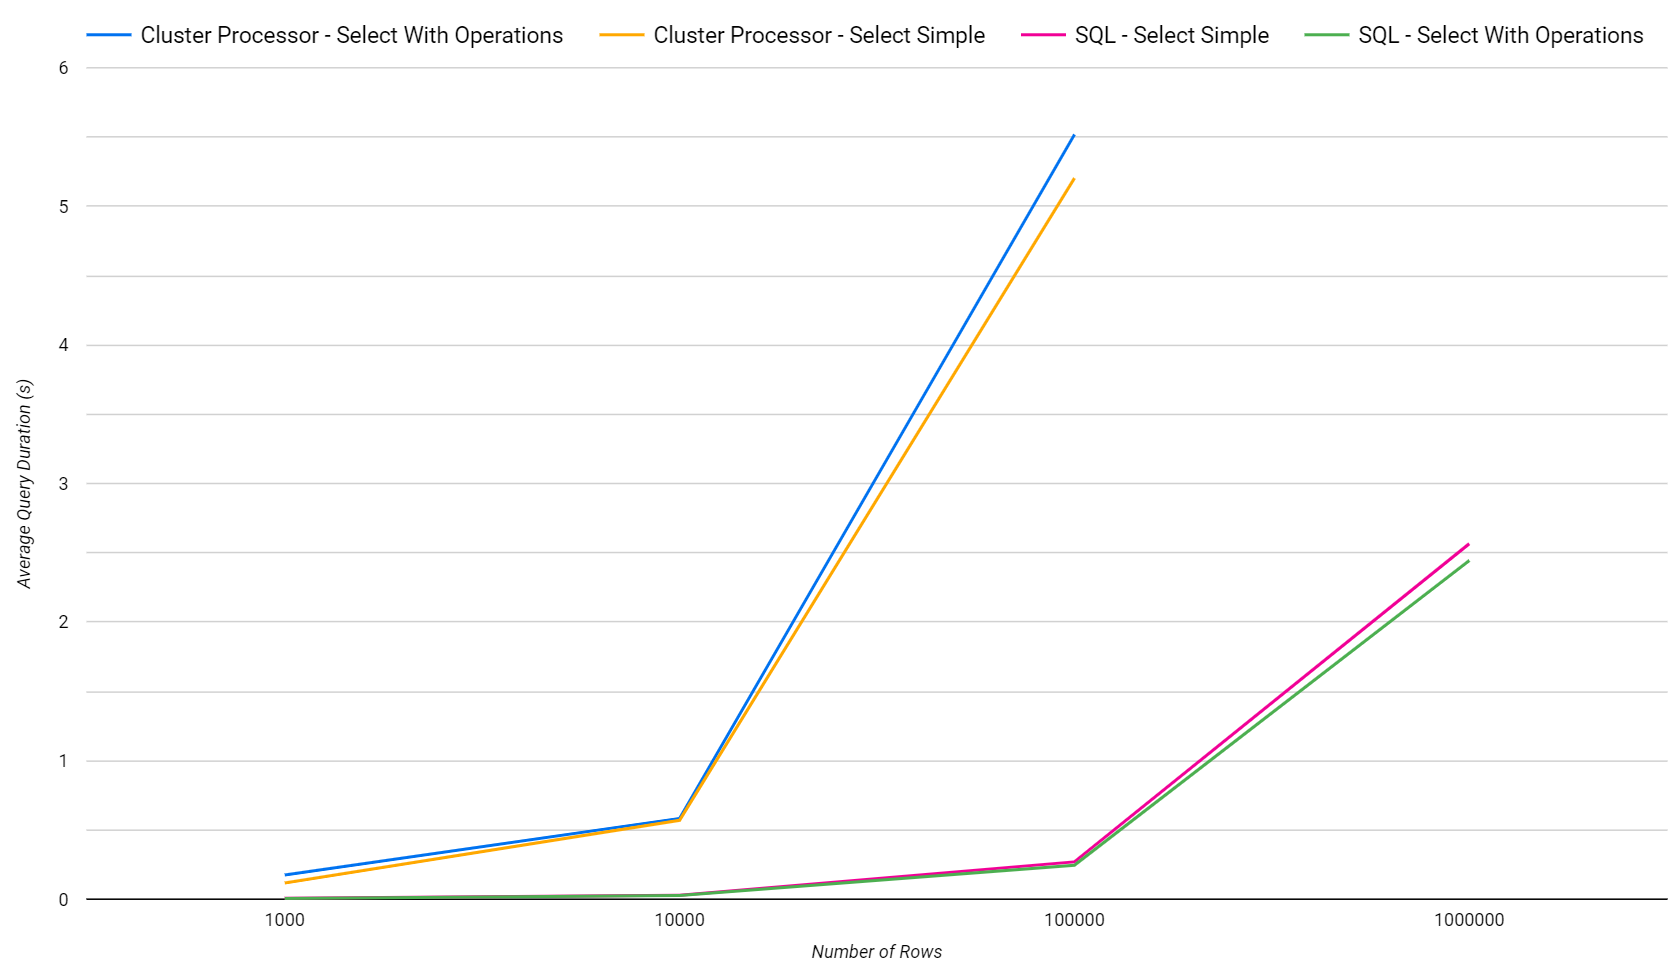
\includegraphics[width=0.8\linewidth]{chapters/diagrams/testing/select-simple-1k-1m}
	\caption{SQL vs Cluster Processor - Select Query Results}
	\label{fig:select-graph}
\end{figure}

\pagebreak
\subsection{Filter Query}
The first query is a simple filter, with no AND/OR combinations. 
%Figures \ref{fig:sql-filter-simple} and \ref{fig:cluster-filter-simple} show the queries. 
The second filter is more complex, testing both boolean operators. 
%Figures \ref{fig:sql-filter-complex} and \ref{fig:cluster-filter-complex} show the queries.

\paragraph{Results}
The results for this query are shown in Figure \ref{fig:filter-graph}. SQL is around 15-20x faster in this test case, which is likely to be partially caused by the transmission format, as with the Select test. However, SQL is likely able to exploit caching more extensively over repeated tests when compared to the Cluster Processor, particularly with smaller tables that can be held in-memory permanently. Conversely, the Cluster Processor fetches fresh data from Cassandra every time the query is called.

The complex Filter reliably executes faster than the simple Filter across all results in both environments.
%For the Cluster Processor, it is nearly 2 seconds faster on average at 10 million rows, and for SQL it is almost 6 seconds faster at 100 million rows. 
This is expected, since the complex filter is more restrictive in the results that it returns, resulting in less data transferred over the network.

\begin{figure}[htp]
	\centering
	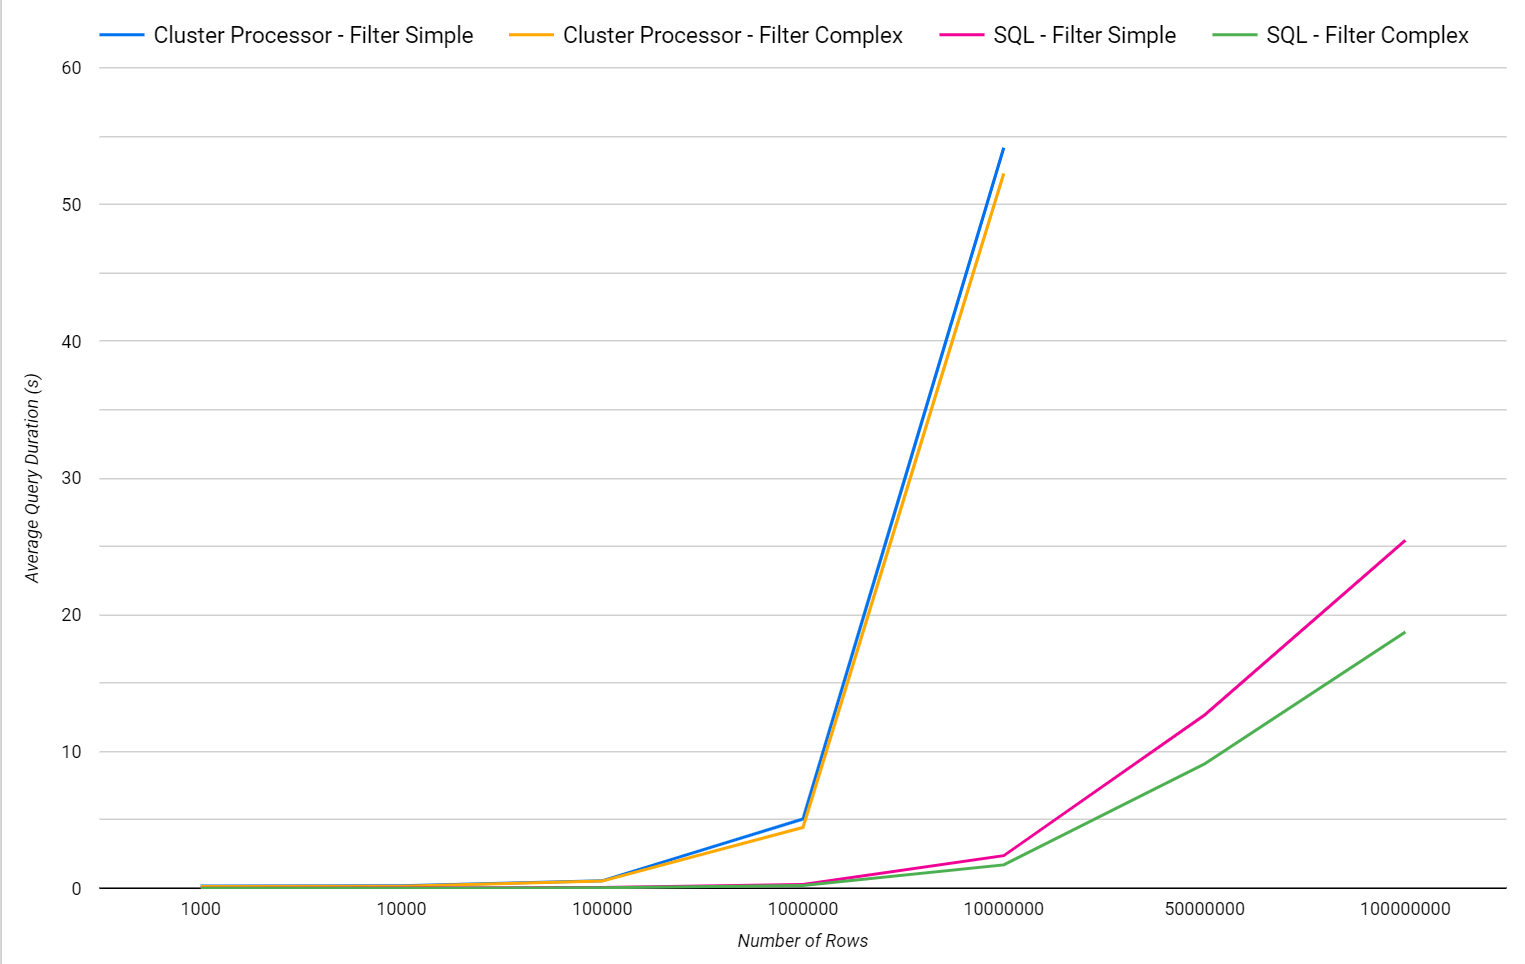
\includegraphics[width=0.8\linewidth]{chapters/diagrams/testing/filter-1k-100m}
	\caption{SQL vs Cluster Processor - Filter Query Results} 
	\label{fig:filter-graph}
\end{figure}

\subsection{Group By Query}
The first query is a simple group by, essentially performing a \texttt{DISTINCT} operation. 
%Figures \ref{fig:sql-group-by-simple} and \ref{fig:cluster-group-by-simple} show the queries. 
The second group by is more complex, featuring a number of aggregations. %Figures \ref{fig:sql-group-by-complex} and \ref{fig:cluster-group-by-complex} show the queries. 

\paragraph{Results}
The results for this query are shown in Figure \ref{fig:group-by-graph}. SQL is significantly faster, and scales much better as the data sizes increase. For the Cluster Processor, the aggregate group by is over twice as fast on average than the simple version at 10 million records. The testing was performed sequentially, with no break between tests, so it is unclear why this result is faster. Furthermore, the same difference in computation time is not present at smaller data volumes. This could be caused by the less controlled cloud environment, meaning perhaps some unexpected load was present during the simple test, resulting in slower computation. Another round of testing would need to be performed to determine if this was the case.

Despite this unexpected difference, there is still a significant performance drop-off compared to the results at 1 million records. Analysing the outputs from the workers, the results could not be stored entirely in-memory, resulting in a large amount of computation time being spent swapping partial results to and from disk. Group By operations suffer from memory shortages worse than other types of queries, as around twice the normal data volume is stored at one time: the source data for the Group By, data for the new hashes, and the newly computed group by partitions are all kept in the data store at the same time.

\begin{figure}[htp]
	\centering
	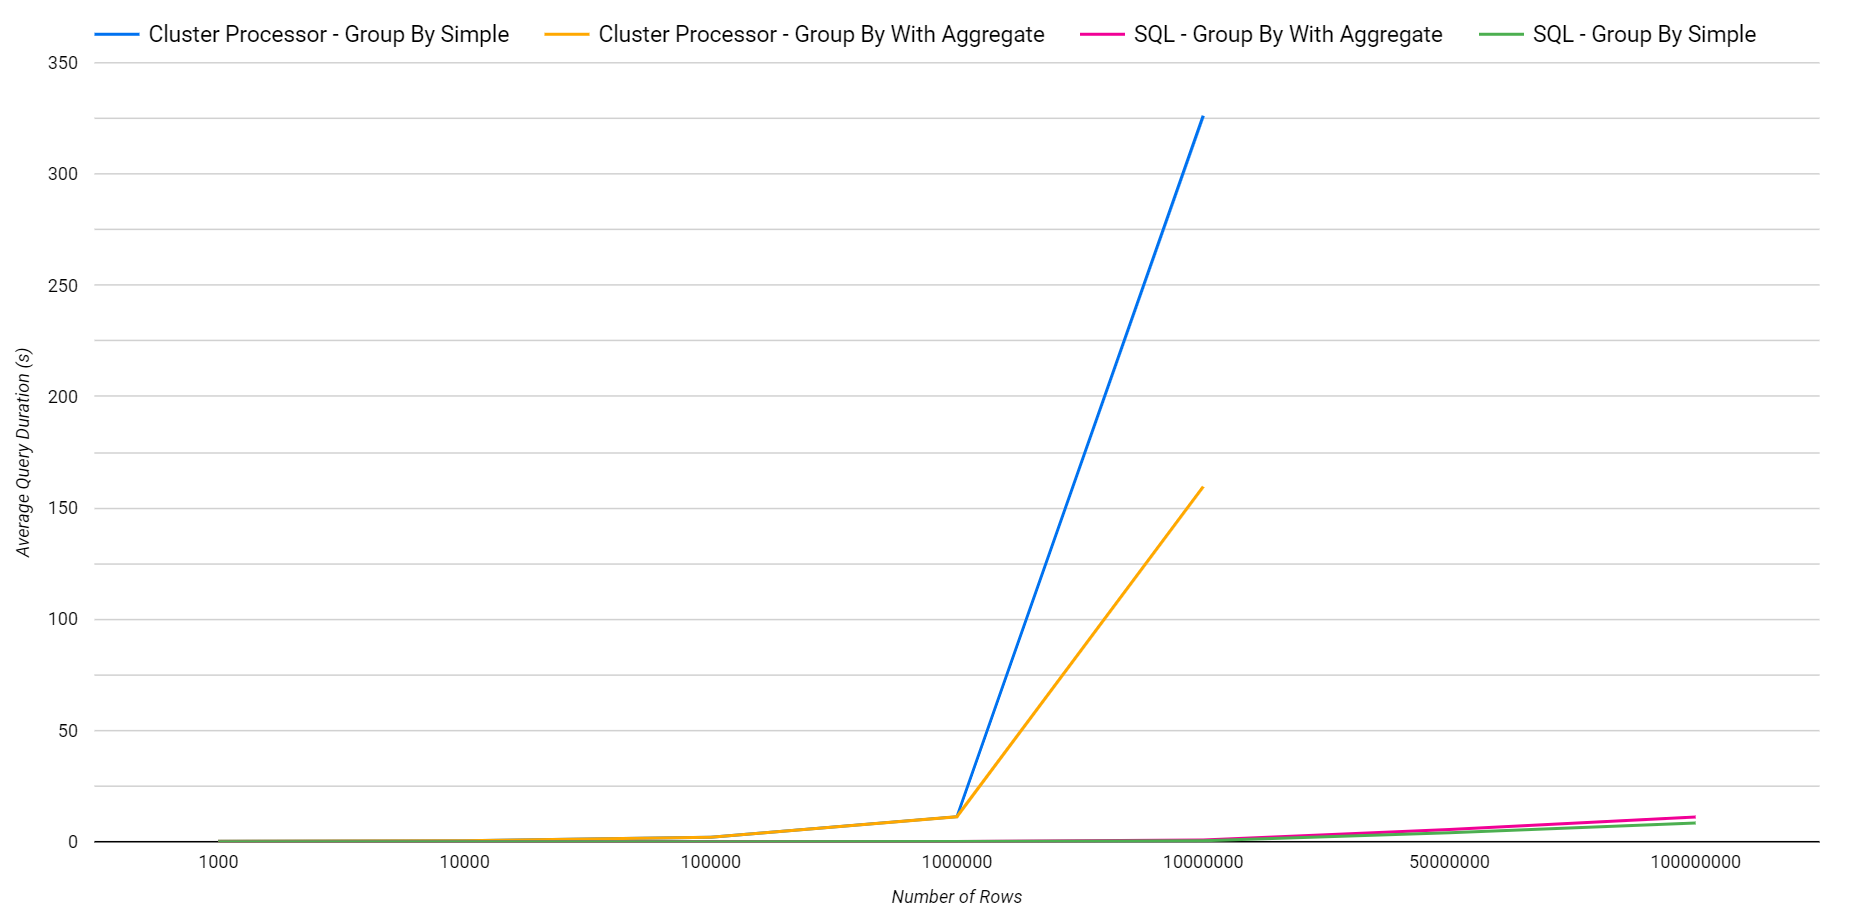
\includegraphics[width=0.8\linewidth]{chapters/diagrams/testing/group-by-1k-100m}
	\caption{SQL vs Cluster Processor - Group By Query Results}
	\label{fig:group-by-graph}
\end{figure}

\subsection{Analysis}\label{subsec:sql-cluster-processor-analysis}
As the raw performance testing results show, a significant amount of optimisation would be required for the Cluster Processor solution to truly compete with SQL with regards to computation speed. The system appears to be weakest at transmitting raw data quickly across the network, and computing Group Bys.

One way to optimise the transmission format for results is to reduce the size of the serialised row data. Currently, every serialised table cell stores value and type information, but types are already sent within the header. Therefore, the system could reduce the serialised size by only sending values, and using the header to perform type casts.

% What's the impact of the calculations, and what's the impact of the network on the results?
The main inefficiency causing the poor Group By performance is the workers holding onto more data than necessary. Currently, the hashing process stores a copy of the entire result before cross-communication occurs. It should be possible to partially perform the Group By operation for each partition on each worker, then finalise the partial results when the partition is computed, significantly reducing the amount of stored and transferred data. As testing has already established that the transmission format is suboptimal, by sending more data than is required, the network inefficiencies have an increased impact on performance. 

Furthermore, when computing Group Bys at 10 million rows, the workers ran low on memory, and began spilling data to disk, which is significantly slower than in-memory storage. By storing less data, spilling would occur at larger data volumes, improving the overall performance.



\section{Level of Parallelisation}\label{sec:parallelisation-test}
This section will compare the performance of the Cluster Processor when the number of workers is changed, but the overall available resources is the same. The aim is to determine how changing the level of parallelisation in the cluster impacts the computation speed. 

In these tests the simple versions of each query type were executed, with different data volumes depending on the test. See Appendix \ref{sec:testing-figs} for query details. 

Figure \ref{fig:parallelisation-test-workers} shows the cluster layouts for each test case; the number of workers, and the resources available to each worker. As shown, the overall number of vCores and GB of memory available to the cluster is the same in each case. 

Throughout all of these tests, the number of Cassandra nodes in the cluster remained consistent: 3 nodes, one placed on each Kubernetes node.

\begin{figure}[ht]
	\centering
	\begin{tabular}{| c | c | c | c | c |}
		\hline
		\textbf{Workers} & \textbf{vCores} & \textbf{Worker Memory} & \textbf{Total vCores} & \textbf{Total Memory} \\ \hline
		2 & 3 & 9GB & 6 & 18GB \\ \hline
		3 & 2 & 6GB & 6 & 18GB \\ \hline
		6 & 1 & 3GB & 6 & 18GB \\ \hline
		9 & 0.666 & 2GB & 6 & 18GB \\ \hline
		12 & 0.5 & 1.5GB & 6 & 18GB \\ \hline
	\end{tabular}
	\caption{Parallelisation - Number of Workers and Resources}
	\label{fig:parallelisation-test-workers}
\end{figure}

\pagebreak
\subsection{Select Query}
The results of this test are shown in Figure \ref{fig:select-simple-parallelisation-test}. Due to the same memory issue as in the SQL test, only 1000 to 100000 row tables were tested. The cluster layout with 3 nodes appears to execute around twice as fast across all data volumes compared to the other layouts, which all have similar execution times on average. It is likely that the extra overhead introduced by the increased parallelisation slowed down data transfer, and there was no computation to perform which would benefit the increased number of nodes. 

However, at 100,000 rows the 9 node cluster ran marginally faster than the other slower layouts. These are still tightly clustered with all results within 0.4s of one another, suggesting this is likely caused by random variation, rather than the 9 node cluster being specifically faster. Further testing, particularly at higher data volumes, would be required to confirm any trends here. 

Interestingly, the 2 node cluster performed slower than the 3 node cluster, likely because this layout has less workers than Cassandra nodes. This adds latency when importing data from the Cassandra node without a co-located worker. 

\begin{figure}[ht]
	\centering
	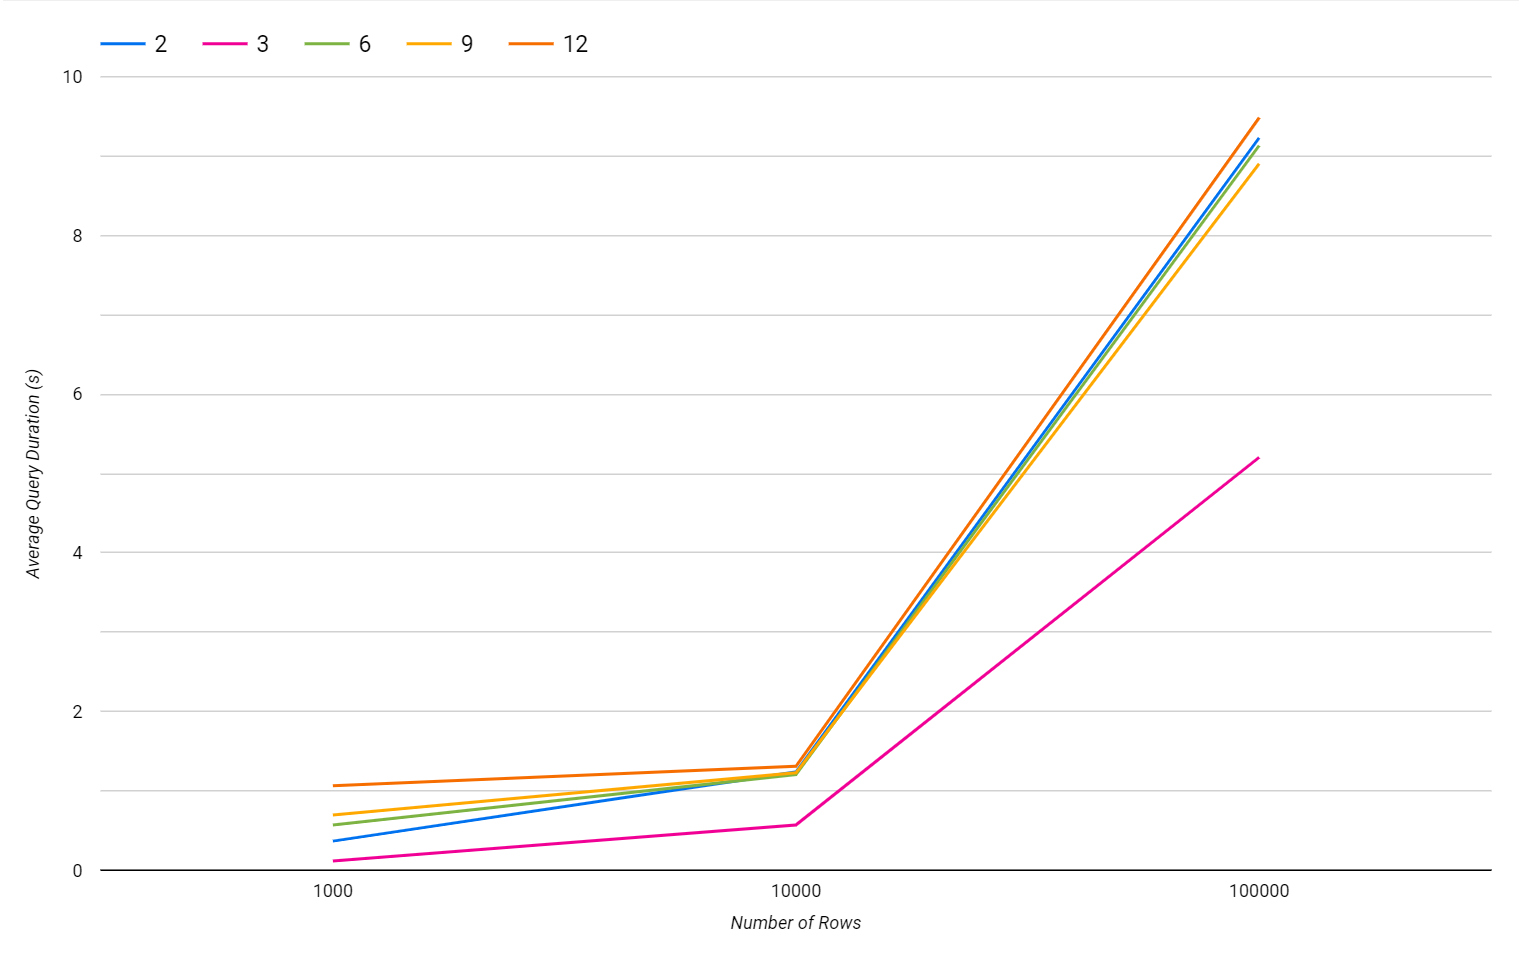
\includegraphics[width=0.8\linewidth]{chapters/diagrams/testing/select-simple-parallelisation-test}
	\caption{Parallelisation - Select Query Results} 
	\label{fig:select-simple-parallelisation-test}
\end{figure}

\pagebreak
\subsection{Filter Query}
The results of this test are shown in Figure \ref{fig:filter-simple-parallelisation-test}. The 3 node cluster is fastest until 100,000 rows, but is then overtaken by the 9 node cluster, showing an interesting trend.

To investigate this trend further, the test was also run for all cluster layouts at 10 million rows, shown in Figure \ref{fig:filter-simple-parallelisation-10m}. The larger clusters (6, 9 and 12 nodes) are all faster than the 3 node cluster, with 9 nodes executing quickest. This shows that as the amount of work increases, the increased level of parallelisation becomes a benefit. The fact that 12 nodes is slower than 9 suggests there is an optimal point that maximises parallelisation without introducing too much overhead from the number of nodes.

\begin{figure}[ht]
	\centering
	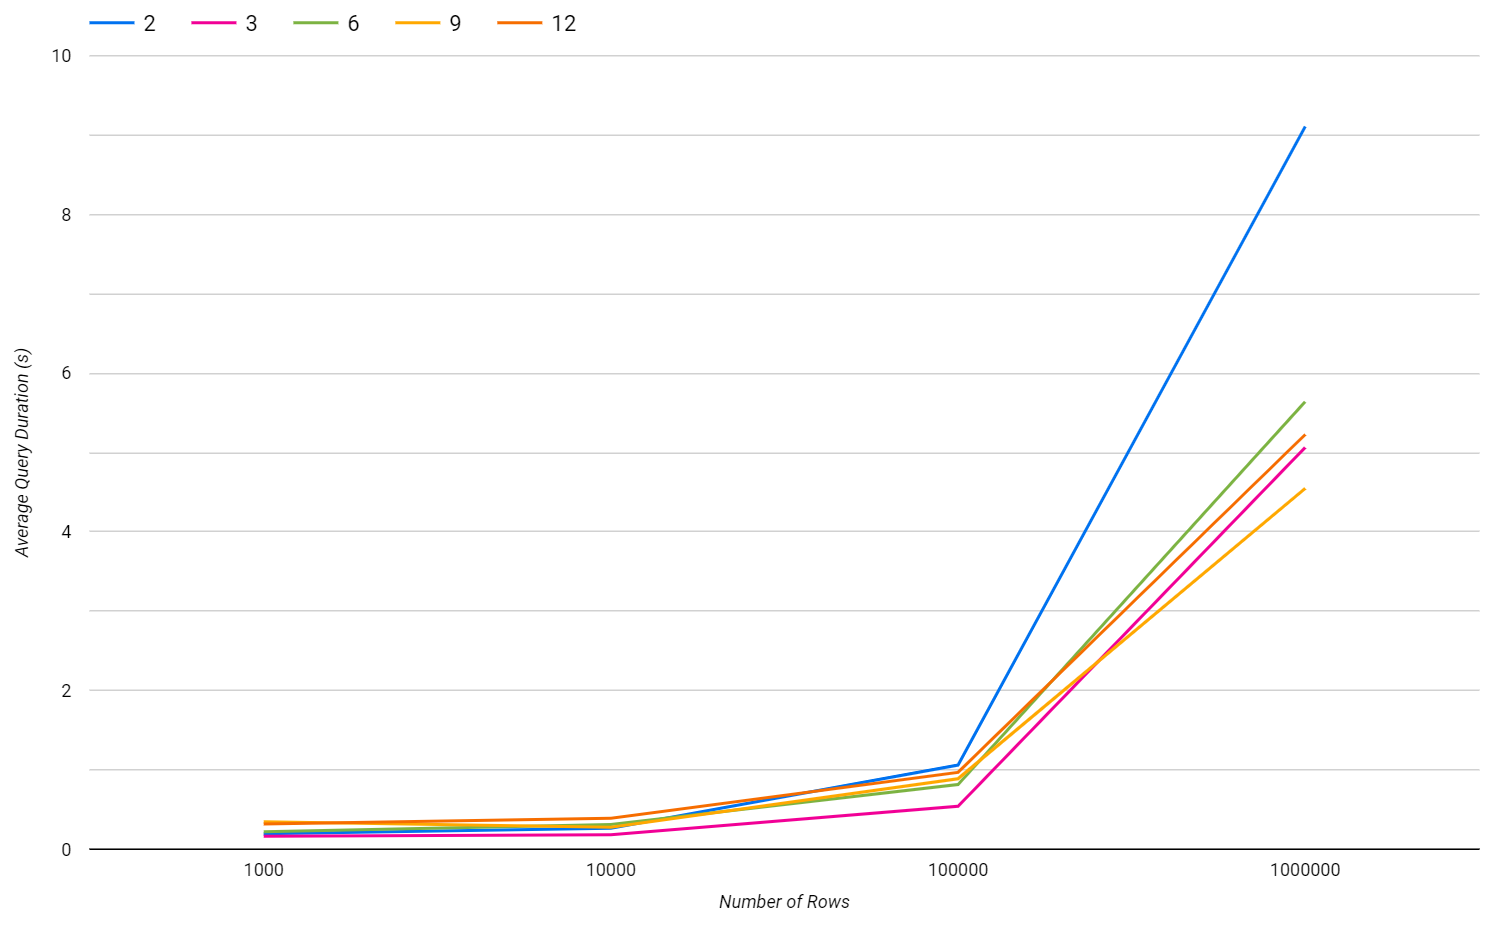
\includegraphics[width=0.8\linewidth]{chapters/diagrams/testing/filter-simple-parallelisation-test}
	\caption{Parallelisation - Filter Query Results}
	\label{fig:filter-simple-parallelisation-test}
\end{figure}

\begin{figure}[ht]
	\centering
	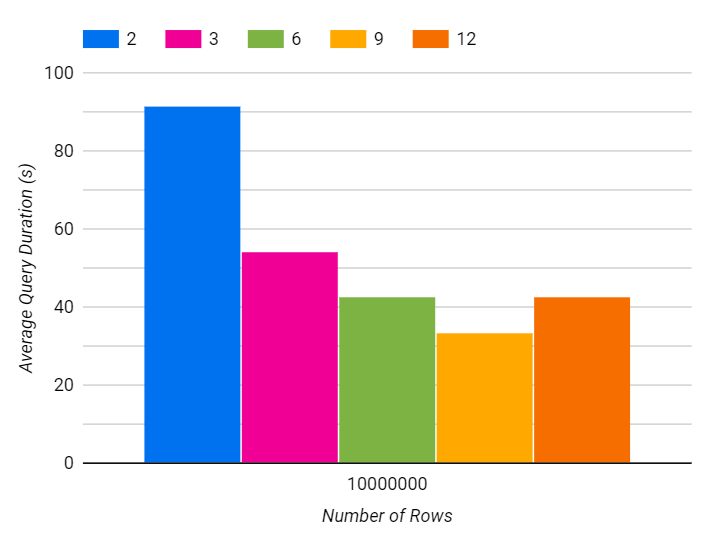
\includegraphics[width=0.4\linewidth]{chapters/diagrams/testing/filter-simple-parallelisation-10m}
	\caption{Parallelisation - Filter Query Results, 10 Million Rows}
	\label{fig:filter-simple-parallelisation-10m}
\end{figure}

\pagebreak
\subsection{Group By Query}
The results of this test are shown in Figure \ref{fig:group-by-simple-parallelisation-test}. They again suggest that there is a balancing point for the level of parallelisation. The 3 node cluster is consistently faster than all other layouts. The larger layouts may be slower because the increased parallelisation introduces more cross-communication, which is slower than local execution.

Interestingly, the 2 node cluster is second fastest until 1 million rows, when its performance significantly reduces. This is likely to be because the increased memory demands on each worker resulted in some results being spilled.

\begin{figure}[ht]
	\centering
	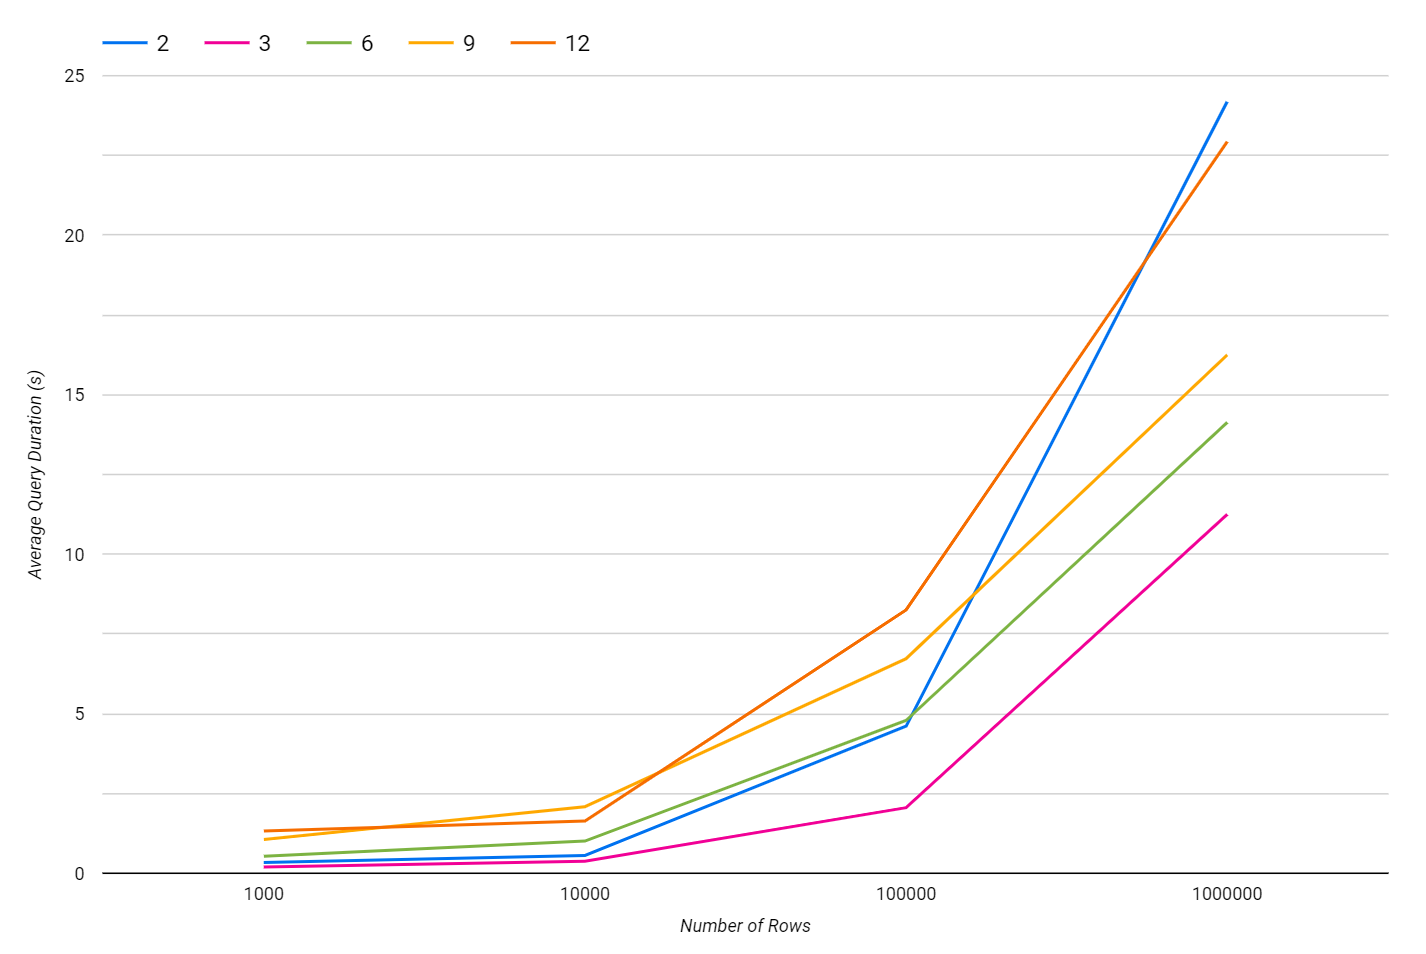
\includegraphics[width=0.8\linewidth]{chapters/diagrams/testing/group-by-simple-parallelisation-test}
	\caption{Parallelisation - Group By Query Results}
	\label{fig:group-by-simple-parallelisation-test}
\end{figure}

\subsection{Analysis}
The outcomes of this test show that there is no clear solution to the level of parallelisation. As a general rule, having the same number of workers as Cassandra nodes will result in good performance, but the Filter test also shows that increasing parallelisation can result in better performance for the same resources at larger query sizes. 

The best solution depends on the queries and data volumes being calculated. This presents an opportunity for further research designing a system that analyses the queries being executed, automatically adjusting the cluster layout to match the requirements of those queries.

\pagebreak
\section{Autoscaling}
This section will compare computation speed of the Cluster Processor when reducing the overall performance, motivated by the autoscaling feature present in many cloud services, including Azure Kubernetes Service. It continually analyses the load of the Kubernetes cluster, changing the number of physical nodes based on current demand \cite{aksautoscaling}. By doing this, applications with fluctating demand can save costs by reducing the number of machines they pay for when demand is low.

While the Cluster Processor would not currently support autoscaling, this test aims to identify the effectiveness of autoscaling on this solution. In these tests the simple versions of each query type were executed, with different data volumes depending on the test. See Appendix \ref{sec:testing-figs} for query details. 

Figure \ref{fig:autoscale-test-workers} shows the cluster layouts for each test case. Each layout has one less worker, and 33\% less resources.

Throughout all of these tests, the number of Cassandra nodes in the cluster remained consistent: 3 nodes, one placed on each Kubernetes node.

\begin{figure}[ht]
	\centering
	\begin{tabular}{| c | c | c | c | c |}
		\hline
		\textbf{Workers} & \textbf{vCores} & \textbf{Worker Memory} & \textbf{Total vCores} & \textbf{Total Memory} \\ \hline
		3 & 2 & 6GB & 6 & 18GB \\ \hline
		2 & 2 & 6GB & 4 & 12GB \\ \hline
		1 & 2 & 6GB & 2 & 6GB \\ \hline
	\end{tabular}
	\caption{Autoscaling - Number of Workers and Resources}
	\label{fig:autoscale-test-workers}
\end{figure}

\subsection{Select Query}
The results of this test are shown in Figure \ref{fig:select-simple-autoscale-test}. As expected, the query performance decreases as the number of workers decreases. At 1000 rows the difference between 3 workers and 1 worker is around 0.3s, and at 10000 rows it is 0.9s.

\begin{figure}[ht]
	\centering
	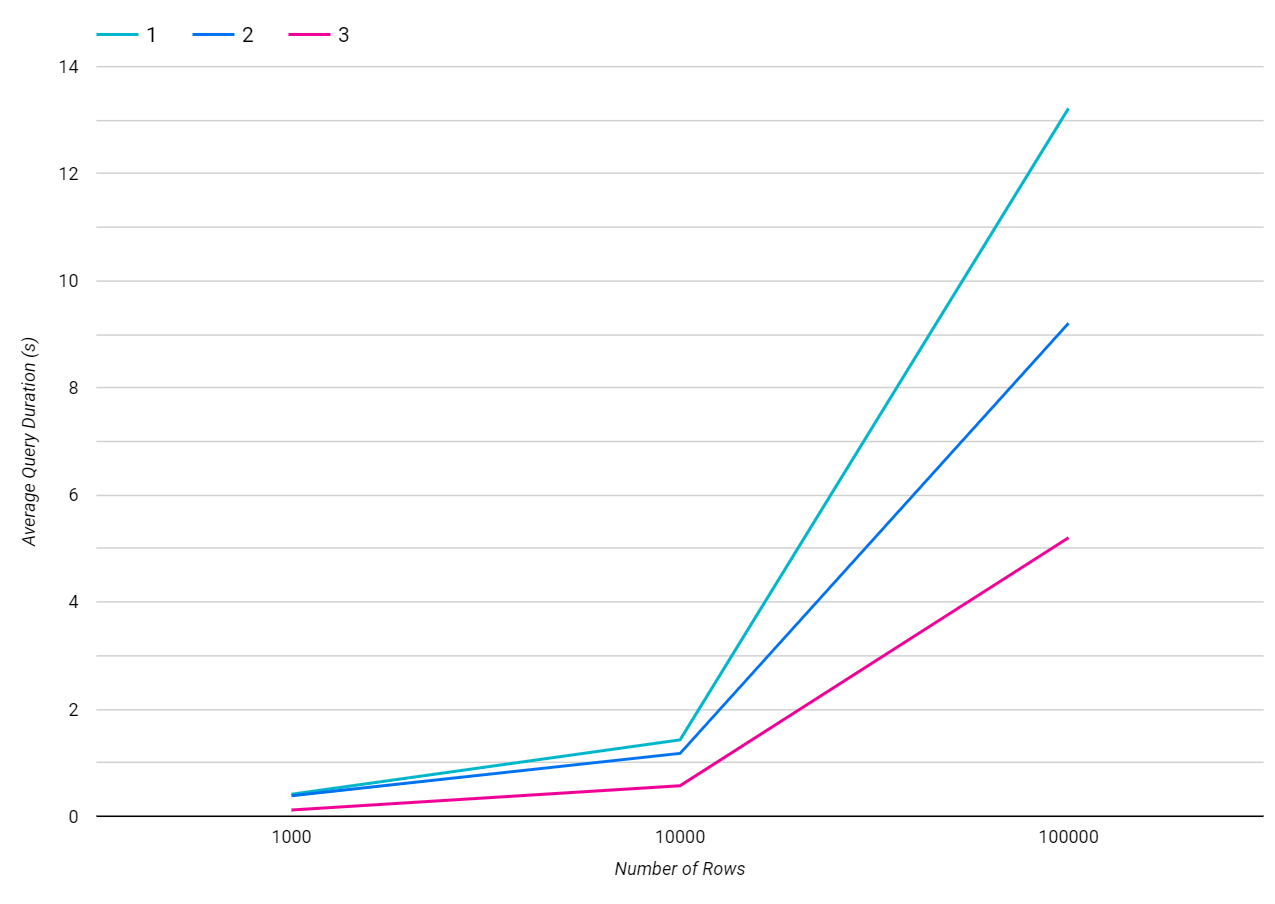
\includegraphics[width=0.7\linewidth]{chapters/diagrams/testing/select-simple-autoscale-test}
	\caption{Autoscaling - Select Query Results}
	\label{fig:select-simple-autoscale-test}
\end{figure}

\subsection{Filter Query}
The results of this test are shown in Figure \ref{fig:filter-simple-autoscale-test}. As before, the query performance decreases with the number of workers. The difference between 1 and 3 workers is 0.08s at 1,000 rows, 0.2s at 10,000 rows, and 1.1s at 100,000 rows.

\begin{figure}[ht]
	\centering
	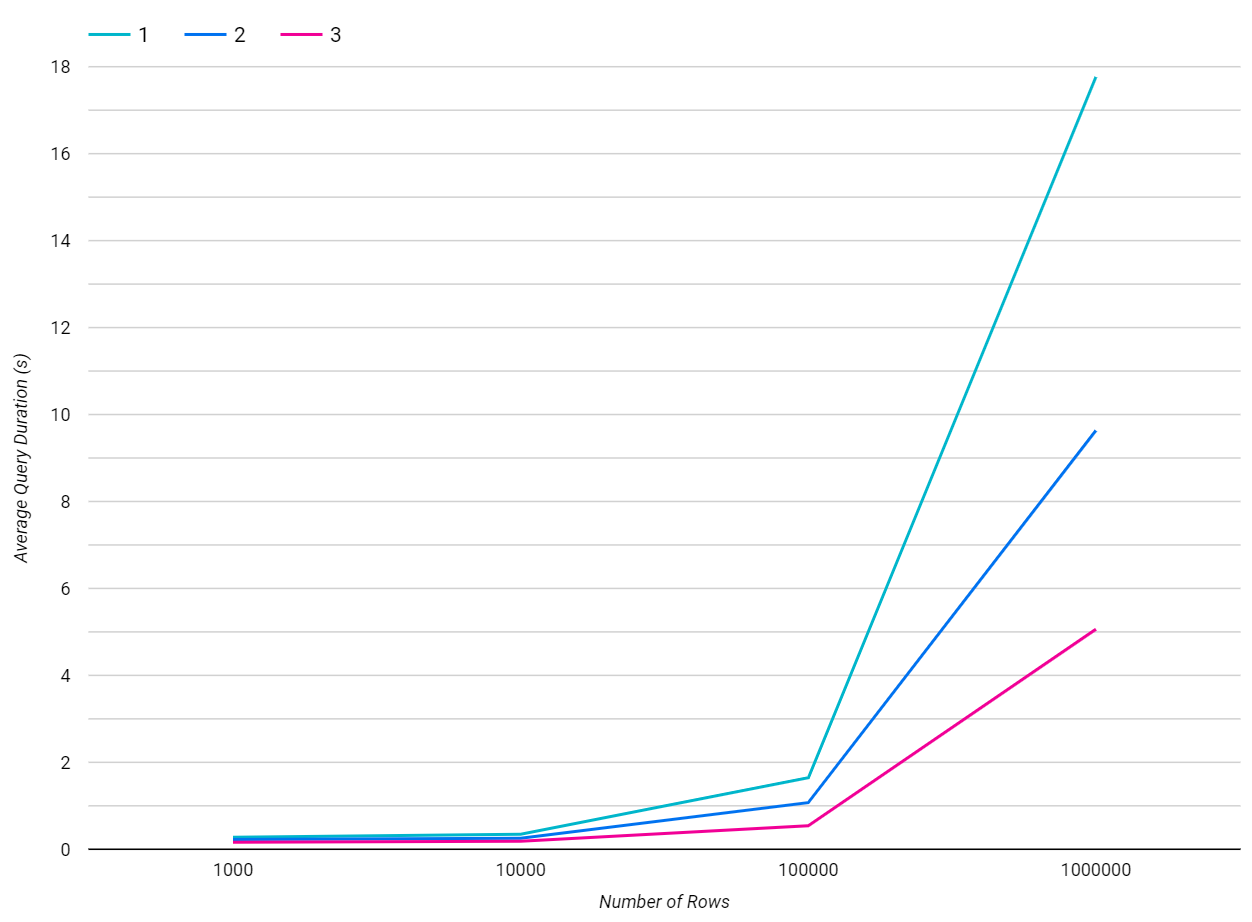
\includegraphics[width=0.8\linewidth]{chapters/diagrams/testing/filter-simple-autoscale-test}
	\caption{Autoscaling - Filter Query Results}
	\label{fig:filter-simple-autoscale-test}
\end{figure}

\pagebreak
\subsection{Group By Query}
The results of this test are shown in Figure \ref{fig:group-by-simple-autoscale-test}. At the two smallest volumes, there is almost no difference between the three layouts, and at 100,000 rows the 1 node cluster is fastest. This suggests that, at very small data volumes, it is faster to perform all of the computation on a single node, as it prevents the need for worker cross-communication.

\begin{figure}[ht]
	\centering
	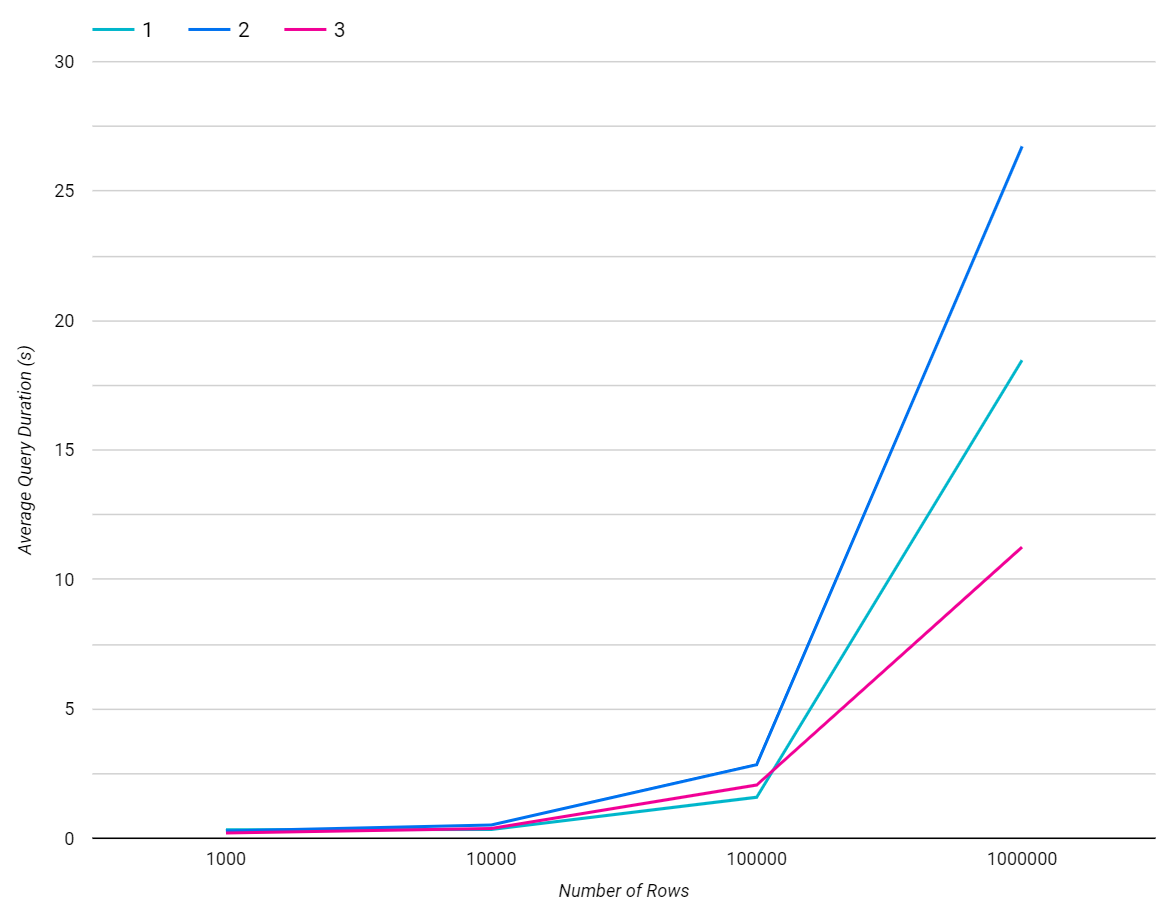
\includegraphics[width=0.8\linewidth]{chapters/diagrams/testing/group-by-simple-autoscale-test}
	\caption{Autoscaling - Group By Query Results}
	\label{fig:group-by-simple-autoscale-test}
\end{figure}

\subsection{Analysis}
The outcomes of this test show that reducing the cluster size is effective at small data volumes. The time difference between the smallest and largest cluster is typically less than a second at less than 1 million rows, which is insignificant for most use cases. If a time-critical system was reliant on querying this amount of data, a single-system solution like SQL would be better suited regardless.
